\documentclass[a4paper,10pt]{article}

\usepackage[utf8]{inputenc}
\usepackage[T1]{fontenc}
\usepackage[english]{babel}

\usepackage{color}
\usepackage{float}
\usepackage{caption}
\usepackage{subcaption}
\usepackage{fancyvrb}

\usepackage{amssymb}
\usepackage{amsmath}
\usepackage{listings}

\usepackage{graphicx}
\DeclareGraphicsExtensions{.png}

\title{DM535 eksamenssæt -- 13. juni 2013 reeksamen \\ \rule{10cm}{0.5mm}}
\author{Studiegruppe F \\ Section S7 \\
DM535\\\rule{5.5cm}{0.5mm}\\}
\date{\today}

\begin{document}

\maketitle

\vfill

\tableofcontents

\newpage

\section{Opgave 1 - Mængder}
a) Betragt de to mængder og afgør, om $S_1 = S_2$.\\\\
$S_1 = (A \cap B \cap C) \cup (B - (A \cup C))$\\
$S_2 = (B - A) \cup (B \cap C)$\\
Hvis vi indtegner vores to mængder i venn diagrammer kan vi sammenligne dem og derudfra konkludere at mængderne ikke er ens. \\
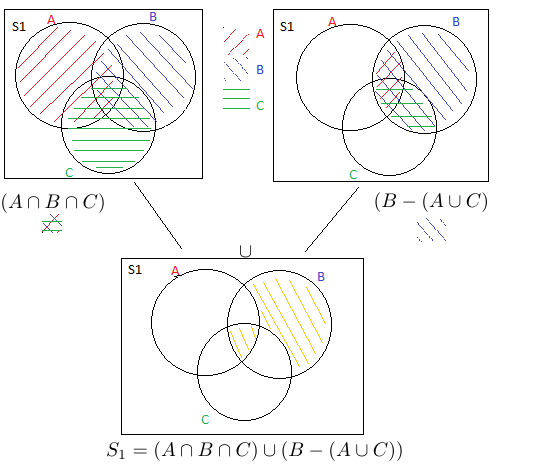
\includegraphics[scale=1]{VennDiagram1.png} 
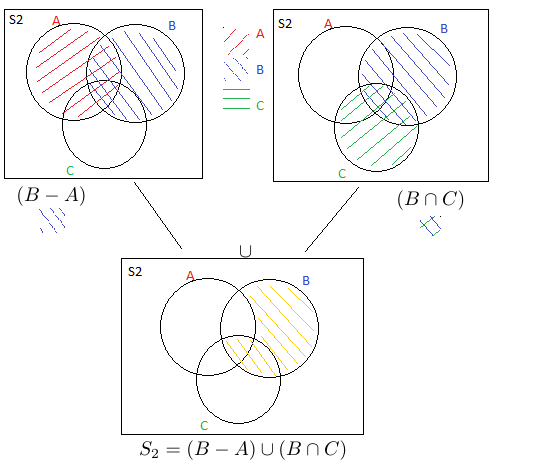
\includegraphics[scale=1]{VennDiagram2.png} 
b) Er følgende udsagn sandt?\\\\
Hvis $A$ og $B$ er tælleligt uendelige mængder, da er $A \cap B$ også tælleligt uendelig.
Udsagnet er falsk, da fællesmængden af $A$ og $B$ ikke nødvendigvis er uendelig. Mængden er dog tællelig da snittet er en delmængde af både $A$ og $B$. Hvis enten $A$ er en delmængde af $B$, eller $B$ en delmængde af $A$ er mængden tælleligt uendelig. Men hvis $A$ repræsenterer de lige tal og $B$ de ulige tal, er fællesmængden 0, og dermed endelig. 
\section{Opgave 2 - Betragt Funktionerne}
Betragt funktionerne $f: \mathbb{R} \rightarrow \mathbb{R}$ og $g: \mathbb{R} \rightarrow \mathbb{R}$ defineret ved.
\begin{align*}
f(x) = x^2+1\\
g(x) = x-1
\end{align*}
a) Angiv $f \cdot g$
\begin{align*}
f \cdot g &= (x^2+1)\cdot (x-1)\\
&= x^3-x^2+x-1
\end{align*}
b) Angiv $g \circ f$
\begin{align*}
g \circ f &= ((x^2+1)-1)\\
&= x^2
\end{align*}
c) Angiv $f \circ f$
\begin{align*}
f \circ f &= (x^2+1)^2+1\\
&= x^4+2x^2+2
\end{align*}
\section{Opgave 3 - Kongruenssystem}
Angiv samtlige løsninger til nedenstående kongruenssystem
\begin{align*}
x \equiv 2 (\bmod 3)\\
x \equiv 3 (\bmod 4)\\
x \equiv 4 (\bmod 5)
\end{align*}
\begin{align*}
m &= 3 \cdot 4 \cdot 5 = 60\\
x &\equiv 2 (\bmod 3) = \{2,5,8,11,14,17,20,23,26,29,32,35,38,41,44,47,50,53,56,59\}\\
x &\equiv 3 (\bmod 4) = \{3,7,11,15,19,23,27,31,35,39,43,47,51,55,59\}\\
x &\equiv 4 (\bmod 5) = \{4,9,14,19,24,29,34,39,44,49,54,59\}
\end{align*}
$x = 59$ er en løsning\\
Løsningsmængden er $\{59+60k\,|\,k \in \mathbb{Z}\} = \{...,-60,-1,59,119,179,...\}$

\section{Opgave 4 - Matrice Induktionsbevis}
a) Betragt matricerne $A = \begin{bmatrix}
0 & 1 \\ 2 & 3\
\end{bmatrix}$ og $B = \begin{bmatrix}
1 & 2 \\ 3 & 4\
\end{bmatrix}$\\
Beregn $A + B$.
\begin{align*}
A + B = \begin{bmatrix}
0 & 1 \\ 2 & 3\ \end{bmatrix} +
\begin{bmatrix}
1 & 2 \\ 3 & 4\
\end{bmatrix} = \begin{bmatrix}
1 & 3 \\ 5 & 7\
\end{bmatrix}
\end{align*}
b) For ethvert $ i \in \mathbb{N}$, lad $A_i = \begin{bmatrix}
i & i+1 \\ i+2 & i+3
\end{bmatrix}$\\
Vis at alle tal i matricen $A_i + A_i+1$ er positive ulige tal, for alle $i \in \mathbb{N}$\\
Vi viser ovenstående ved hjælp af induktion.\\
Vores basisskridt er at vise $i = 1$
\begin{align*}
A_1+A_{1+1} = \begin{bmatrix}
1 & 1+1 \\ 1+2 & 1+3
\end{bmatrix}+\begin{bmatrix}
1+1 & 1+1+1 \\ 1+1+2 & 1+1+3
\end{bmatrix} = \begin{bmatrix}
3 & 5 \\ 7 & 9
\end{bmatrix}
\end{align*} 
Vi kan se at alle tal i matricen er positive ulige tal og går dermed videre til vores induktionsskridt.\\
Vi antager  $A_i = \begin{bmatrix}
i & i+1 \\ i+2 & i+3
\end{bmatrix}$\\
Vi vil vise $A_i + A_{i+1}$ er positive ulige tal\\
Vores induktionsskridt er at vise at $A_i + A_{i+1}$ også gælder når $ i = i+1 \Rightarrow A_{i+1} + A_{i+2}$
\begin{align*}
A_{i+1}+A_{i+2} &= \begin{bmatrix}
i+1 & i+1+1 \\ i+1+2 & i+1+3
\end{bmatrix}+\begin{bmatrix}
i+2 & i+3 \\ i+4 & i+5
\end{bmatrix}\\ &= \begin{bmatrix}
2i+3 & 2i+5 \\ 2i+7 & 2i+9
\end{bmatrix}
\end{align*}
Vi ved at alle tal $\in \mathbb{N}$ ganget med et lige til giver et lige tal. Dermed afgører konstanten i vores felter i $2x2$ matrice om resultatet er lige eller ulige. Da alle konstanter er ulige medfører dette er ulige tal uanset hvad $i$ er.
Vi har med induktion dermed bevist at: $A_i + A_{i+1}$ er positive ulige tal.\\
c) Hvilke af de seks nedenstående udsagn er ækvivalente med udsagnet, som skulle bevises i spørgsmål b?\\
Udsagn 5 og 6 er ækvivalent med udsanget i spørgsmål b. 
\section{Opgave 5 - Dobbeltsum}
Beregn følgende dobbeltsum
\begin{align*}
\sum_{i=6}^{10} \sum_{j=1}^{i}j
\end{align*}
Den indre sum kender vi en anden formel for og kan omskrives til 
\begin{align*}
\sum_{j=1}^{i}j &= \frac{i(i+1)}{2}
\end{align*}
Den ydre sum kan vi omskrive til noget vi nemmere kan arbejde med
\begin{align*}
\sum_{i=6}^{10} = \sum_{i=1}^{10} - \sum_{i=1}^{5}
\end{align*}
Vi får så at summen er
\begin{align*}
\sum_{i=1}^{10}\frac{i(i+1)}{2} - \sum_{i=1}^{5}\frac{i(i+1)}{2}
\end{align*}
Dette kan omskrives til
\begin{align*}
&\frac{1}{2}\sum_{i=1}^{10}i^2 + \frac{1}{2}\sum_{i=1}^{10}i - \frac{1}{2}\sum_{i=1}^{5}i^2 - \frac{1}{2}\sum_{i=1}^{5}i\\
\end{align*}
Ved opslag i tabel 2 afsnit 4.2 kan vi beregne summen til
\begin{align*}
\frac{1}{2}\left(\frac{10 \cdot 11 \cdot 21)}{6}\right) + \frac{1}{2}\left( \frac{10 \cdot 11}{2} \right)  - \frac{1}{2} \left(\frac{5 \cdot 6 \cdot 11}{6}\right) - \frac{1}{2} \left(\frac{5 \cdot 6}{2} \right)&= \\
192,5 + 27,5 - 27,5 - 7,5 &= 185
\end{align*}
\section{Opgave 6 - Binære relationer}
Spørgsmål a og b handler om binære relationer på mængden $A = \{1,2,3,4,5\}$.\\\\
a) Hvilke relationer i Figur 1 er ækvivalensrelationer?\\
Definitionen på en ækvivalensrelation er at den skal være refleksiv, transitiv og symmetrisk\\
Figur a er ikke en ækvivalensrelation da den ikke er refleksiv, elementet $(1,1)$ er der  f.eks ikke.\\
Figur b er ikke en ækvivalensrelation da den ikke er refleksiv, elementet $(1,1)$ er der  f.eks ikke.\\
Figur c er en ækvivalensrelation da den er refleksiv, transitiv og symmetrisk.
Figur d er ikke en ækvivalensrelation da den ikke er refleksiv, elementet $(1,1)$ er der  f.eks ikke.\\
Figur e er ikke en ækvivalensrelation da den ikke er symmetrisk, f.eks er elementet $(1,3)$ der men $(3,1)$ er der ikke.\\
Figur f er ikke en ækvivalensrelation da den ikke er refleksiv, elementet $(1,1)$ er der f.eks ikke.\\\\
b) Hvilke relationer i Figur 1 er partielle ordninger?\\
Definitionen på en Partielle ordninger er at den skal være refleksiv, transitiv og antisymmetrisk\\
Figur a er ikke en partiel ordning da den ikke er refleksiv, elementet $(1,1)$ er der  f.eks ikke.\\
Figur b er ikke en partiel ordning da den ikke er refleksiv, elementet $(1,1)$ er der  f.eks ikke.\\
Figur c er ikke en partiel ordning da den ikke er antisymmetrisk både $(1,4)$ og $(4,1)$ er repræsenteret.
Figur d er ikke en partiel ordning da den ikke er refleksiv, elementet $(1,1)$ er der  f.eks ikke.\\
Figur e er ikke en partiel ordning da den ikke er transitiv. Man kan komme fra $1$ til $5$ og $5$ til $4$ men ikke fra $1$ til $4$.\\
Figur f er ikke en partiel ordning da den ikke er refleksiv, elementet $(1,1)$ er der f.eks ikke.\\\\
c) Betragt nu følgende ækvivalensrelation på $\mathbb{Z}$
\begin{align*}
R = \{(a,b)\,|\,a+b \equiv 0\,\,\, (\bmod 2) \}
\end{align*}
Angiv alle elementer i ækvivalensklassen for 3, d.v.s $[3]_R$.
\begin{align*}
[3]_R &= [1]_R = [c]_R \,\, \text{,hvor c er et ulige tal i } \mathbb{Z}\\
[3]_R &= \{...,-5,-3,-1,1,3,5,...\} = \{n+1\,|n \in \mathbb{Z}\}
\end{align*}
\end{document}